\subsection{Tijd en Wektijd}

\subsubsection{Gedrag}
Na een reset of bij het veranderen van de minuten zal de entity tijd data gaan verzenden. De data die verzonden wordt bevat informatie over welk character geprint moet worden en zijn positie. De characters die moeten worden verzonden worden bepaalt aan de hand van de minuten en uren die de entity in gaan. Dit zal altijd op de volgende volgorde gaan: tientallen uren, eentallen uren, tientallen minuten en als laatste eentallen minuten. Ook zal de module bij een opgaande flank van het \'e\'en Hz signaal de dubbele punt tussen de uren en minuten aan of uit zetten.\\
Het component wektijd verzend dezelfde informatie naar het LCD, alzij het op een andere positie. De wektijd zal beginnen met verzenden op het moment dat de wektijd wordt aangepast in het menu. De volgorde van de van de wektijd is hetzelfde als die van het component tijd.

\subsubsection{Functionaliteit}
Het component tijd werkt volgens het Moore principe. Om de seconde wordt een nieuw character naar het LCD gestuurd. Dit character is voor de dubbele punt tussen de uren en minuten. Als er een minuut om is dan zal de nieuwe tijd naar het LCD worden verzonden.\\
Het component wektijd werkt ook volgens een Moore principe. Op het moment dat er in het menu de wektijd wordt aangepast zal het component wektijd het LCD blijven updaten met de huidige wektijd, dit om een goede feedback te geven naar de gebruiker.

\subsubsection{FSM}
\begin{figure}[h!]
	\center
	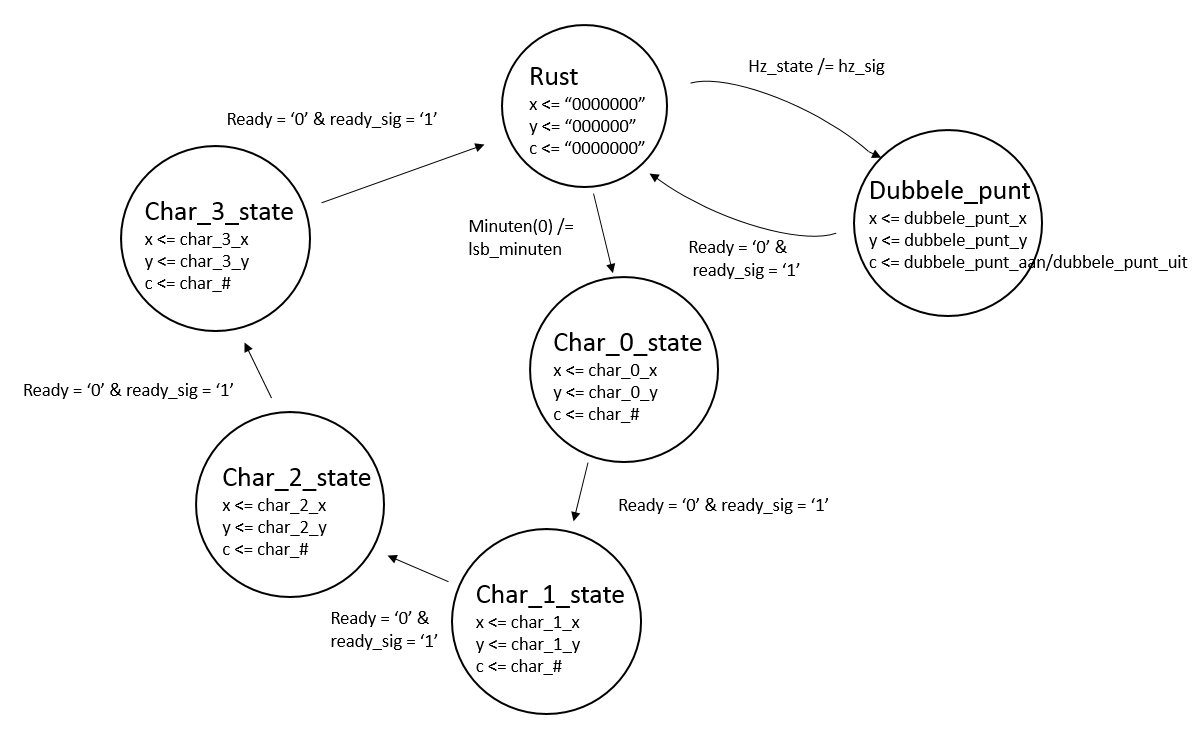
\includegraphics[scale=1.9]{Figuren/LCD/fsm_tijd.png}
	\caption{FSM van component tijd}
	\label{fig:fsm_tijd}
\end{figure}
\begin{figure}[h!]
	\center
	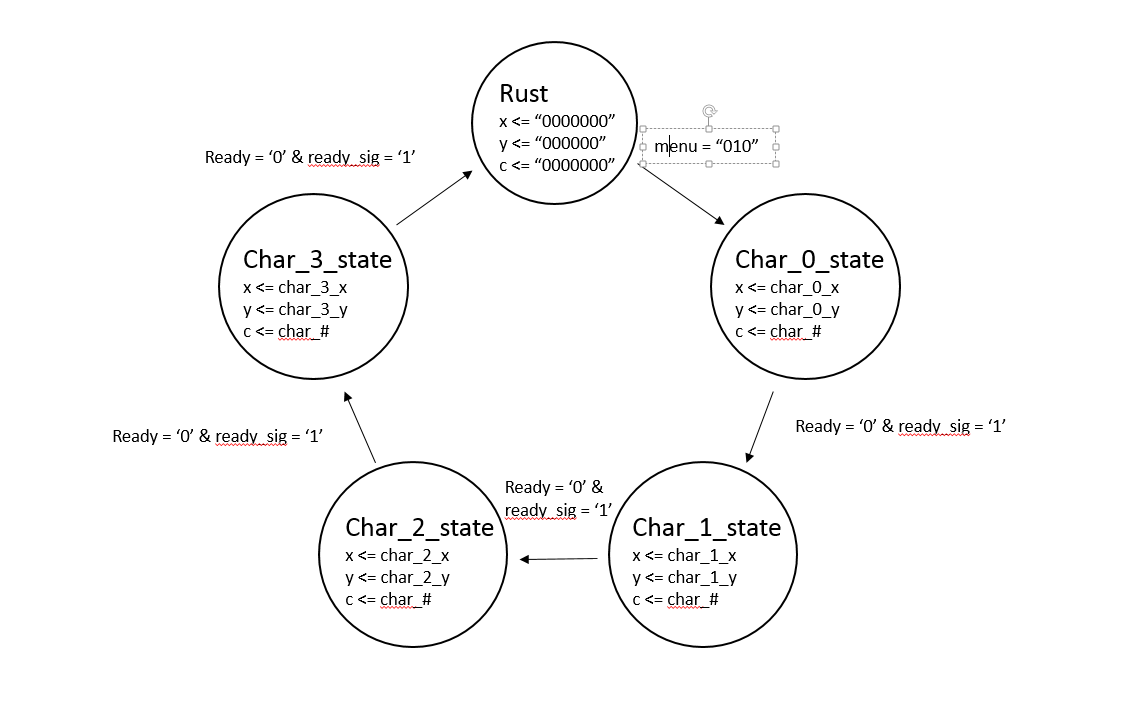
\includegraphics[scale=1.9]{Figuren/LCD/fsm_wektijd.png}
	\caption{FSM van component wektijd}
	\label{fig:fsm_wektijd}
\end{figure}

\subsubsection{VHDL code}
De VHDL code van de tijd is te vinden in appendixes \cite{code:ent_tijd}, \cite{code:beh_tijd}. De VHDL code van de wektijd is te vinden in appendixes \cite{code:ent_wektijd} en \cite{code:beh_wektijd}.

\subsubsection{Simulaties}
Zie \cite{fig:sim_tijd} voor de simulatie resultaten van de tijd. Deze simulatie is met de testbench gedaan die te vinden is in \cite{code:tb_tijd}.\\
De simulatie resultaten van de wektijd is te vinden in \cite{fig:sim_wektijd}. Deze simulatie is met de testbench gedaan die te vinden is in \cite{code:tb_wektijd}.

\subsubsection{Resultaten}
De simulatie resultaten van allebei de componenten zijn zoals die te verwachten zijn. Hierdoor kunnen we concluderen dat allebei de componenten naar behoren werken.


